\documentclass[oneside, 12pt, a4paper]{article}
\usepackage{amsmath}
\usepackage{graphicx}
\usepackage{fancyhdr}
\usepackage{geometry}
\usepackage{hyperref}
\usepackage{lastpage}

\usepackage{natbib}
\bibliographystyle{unsrtnat}

\geometry{a4paper, top = 22mm, left = 25mm, right = 15mm, bottom = 25mm}
\setlength{\headheight}{28pt}

\pagestyle{fancy}
% Create Header for all non-title pages
\fancyhead[L]{
Lorem Ipsum Corp.\\
22/JAN/2021}
\fancyhead[C]{Lorem Ipsum - Report \\}
\fancyhead[R]{
\includegraphics[height=0.75cm]{gpc-service-logo.png}
}

% Create footer with document meta data
\fancyfoot[R]{Page \thepage\phantom{ }of \pageref*{LastPage}}
\fancyfoot[L]{template\_name\_D01}
\fancyfoot[C]{Effective Date: 01/JAN/1960}

\begin{document}
\begin{titlepage}
   \begin{center}
    
\includegraphics[width=0.6\textwidth]{gpc-service-logo.png}
       \vspace*{1cm}
        \vfill
        \huge
        \textbf{Lorem Ipsum - Report} \\
        \large
        \vspace{0.5cm}
        enter subtitle or leave blank\\
        \vspace{0.5cm}
        Date: 22/JAN/2021\\
        \vspace{1.5cm}
        \vfill
        \vspace{0.8cm}

\begin{flushleft}
Ronald A. Fisher\\
GCP-Service International Ltd. \& Co. KG \\
Anne-Conway-Str. 2 \\
28359 Bremen, Germany \\
E-mail: \href{mailto:rfisher@gcp-service.com}{\nolinkurl{rfisher@gcp-service.com}}\\
Tel +49 (0)421 20 80 98 51
\end{flushleft}
\end{center}

\end{titlepage}

% Add ToC
\tableofcontents
\newpage
\listoffigures
\newpage
% Start of actual document

% body will be replaced by the text that is compiled in the *.rmd file
\hypertarget{this-section-title-is-created-using-rmd-syntax}{%
\section{This Section Title is created using
rmd-syntax}\label{this-section-title-is-created-using-rmd-syntax}}

The following text is filler and can be replaced by real content. I
really recommend having a look at the rmarkdown cheat sheet:
\url{https://rstudio.com/wp-content/uploads/2015/02/rmarkdown-cheatsheet.pdf}
The next is created using LateX!

\section{Some Plot}

Here are some nomally distributed random numbers:

\begin{center}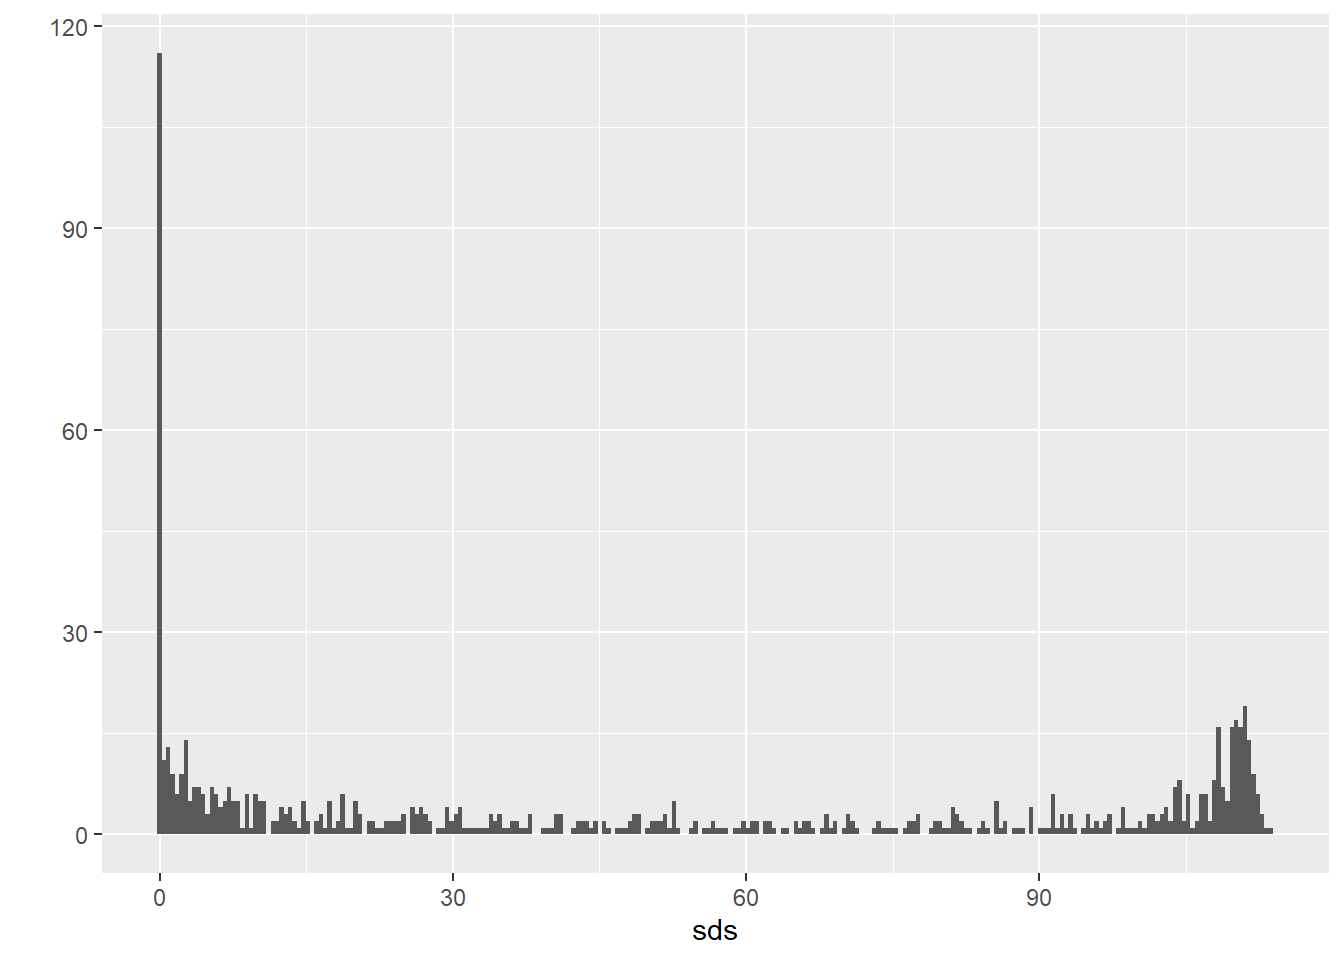
\includegraphics{skeleton_files/figure-latex/unnamed-chunk-2-1} \end{center}

Here is an overview of \(\chi^2\)-distributions with various degrees of
freedom:

\begin{center}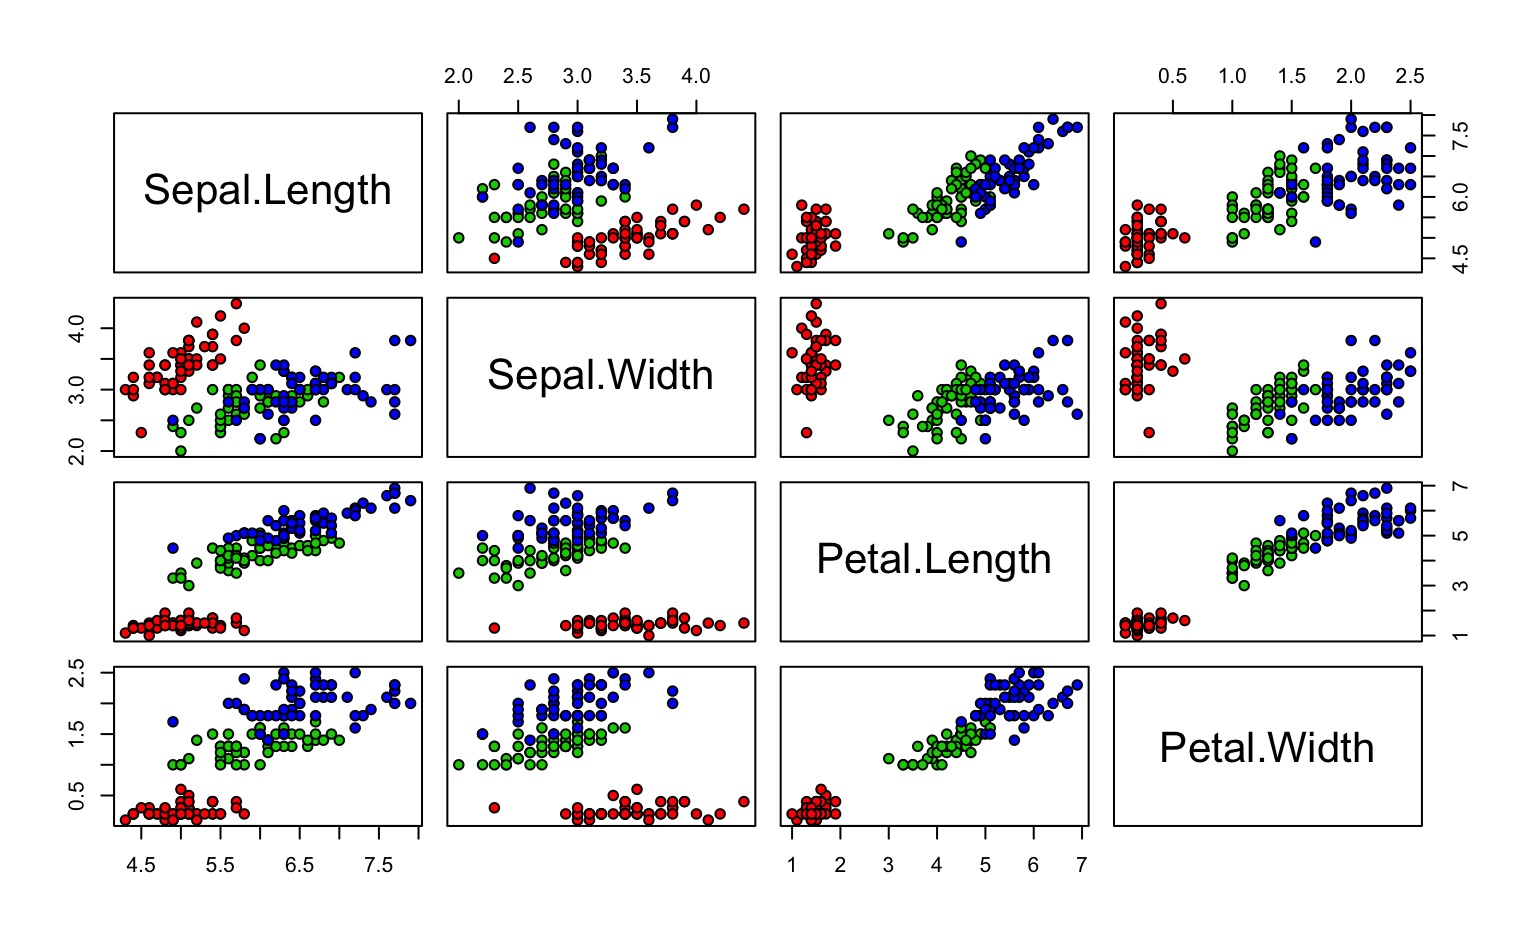
\includegraphics{skeleton_files/figure-latex/unnamed-chunk-3-1} \end{center}

This is the end of this section.

\subsection{Some Text}

Lorem ipsum dolor sit amet, consetetur sadipscing elitr, sed diam nonumy
eirmod tempor invidunt ut labore et dolore magna aliquyam erat, sed diam
voluptua. At vero eos et accusam et justo duo dolores et ea rebum. Stet
clita kasd gubergren, no sea takimata sanctus est Lorem ipsum dolor sit
amet. Lorem ipsum dolor sit amet, consetetur sadipscing elitr, sed diam
nonumy eirmod tempor invidunt ut labore et dolore magna aliquyam erat,
sed diam voluptua. At vero eos et accusam et justo duo dolores et ea
rebum. Stet clita kasd gubergren, no sea takimata sanctus est Lorem
ipsum dolor sit amet.

\subsection{Some Maths}

Here is a model: \begin{align}
Y = \beta_0 + \beta_1 X_i + \epsilon \\
Y_i = \beta_0 + \beta_1 X_i + \epsilon_i ,
\end{align} and here is some unnumbered equation: \begin{align*}
a^2 + b^2 = c^2
\end{align*}

\section{Conclusion}

This is a nice template, says Fisher \cite{fisher_statistical_1970}
(Acutally, he doesn't. I just wanted to show a way of adding
literature).

\newpage
\addcontentsline{toc}{Chapter}{References}
\bibliography{references}
\end{document}
